\documentclass{article}
\usepackage{graphicx}
\usepackage{float}
\usepackage{xcolor}
\usepackage{listings}

\definecolor{mGreen}{rgb}{0,0.6,0}
\definecolor{mGray}{rgb}{0.5,0.5,0.5}
\definecolor{mPurple}{rgb}{0.58,0,0.82}
\definecolor{backgroundColour}{rgb}{0.95,0.95,0.92}

\lstdefinestyle{CStyle}{
    backgroundcolor=\color{backgroundColour},   
    commentstyle=\color{mGreen},
    keywordstyle=\color{magenta},
    numberstyle=\tiny\color{mGray},
    stringstyle=\color{mPurple},
    basicstyle=\footnotesize,
    breakatwhitespace=false,         
    breaklines=true,                 
    captionpos=b,                    
    keepspaces=true,                 
    numbers=left,                    
    numbersep=5pt,                  
    showspaces=false,                
    showstringspaces=false,
    showtabs=false,                  
    tabsize=2,
    language=C
}

\title{File transfer ove TCP/IP in CLI}
\date{5/3/2020}
\author{Distributed System Group 4}

\begin{document}
\maketitle
\pagenumbering{gobble}
\newpage
\tableofcontents
\newpage
\pagenumbering{arabic}
\section{Introduction}
    If we are creating a connection between client and server using TCP then it has few functionality like, TCP is suited for applications that require high reliability, and transmission time is relatively less critical. It is used by other protocols like HTTP, HTTPs, FTP, SMTP, Telnet. TCP rearranges data packets in the order specified. There is absolute guarantee that the data transferred remains intact and arrives in the same order in which it was sent. TCP does Flow Control and requires three packets to set up a socket connection, before any user data can be sent. TCP handles reliability and congestion control. It also does error checking and error recovery. Erroneous packets are retransmitted from the source to the destination.

\section{How we design out Protocol}
    \begin{figure}[H]
    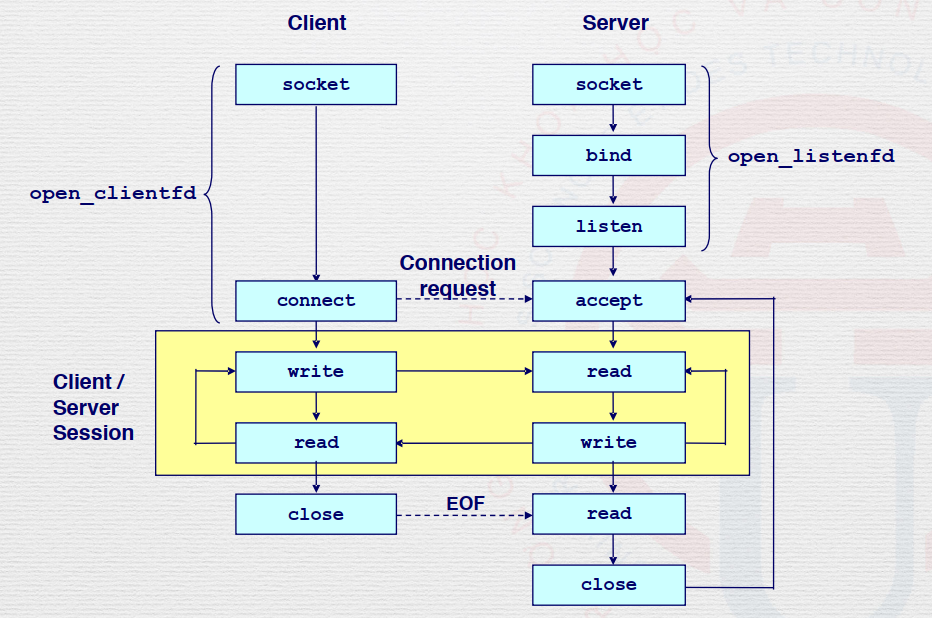
\includegraphics[width=\linewidth]{protocol.png}
    \caption{Protocol}
    \end{figure}


\section{How we organized our System}
    \subsection{Open Session}
    \begin{itemize}
        \item The server socket will be bound to port 8080.
        \item The server socket then listening to y message / data received.
    \end{itemize}

    \subsection{End open listen of server}
    \begin{itemize}
        \item After getting the server socket to listening, the client socket will try to connect to the server.
    \end{itemize}

    \subsection{End open client socket}
    \begin{itemize}
        \item In Client/Server session, both client and server sending eachother messages.
    \end{itemize}



\section{Code}
\subsection{Client}
\begin{lstlisting}[style=CStyle]
    #include <stdio.h>
    #include <stdlib.h>
    #include <unistd.h>
    #include <string.h>
    #include <sys/types.h>
    #include <sys/socket.h>
    #include <netdb.h>

    int main(int argc, char* argv[]) {
        int so;
        char s[100];
        struct sockaddr_in ad;

        socklen_t ad_length = sizeof(ad);
        struct hostent *hep;

        // create socket
        int serv = socket(AF_INET, SOCK_STREAM, 0);
        if (serv == -1) { 
            printf("socket creation failed...\n"); 
            exit(0); 
        } 
        else
            printf("Socket successfully created..\n"); 
        // init address
        hep = gethostbyname(argv[1]);
        memset(&ad, 0, sizeof(ad));
        ad.sin_family = AF_INET;
        ad.sin_addr = *(struct in_addr *)hep->h_addr_list[0];
        ad.sin_port = htons(8080);

        // connect to server
        connect(serv, (struct sockaddr *)&ad, ad_length);

        while (1) {
            // after connected, it's client turn to chat

            // send some data to server
            printf("client>");
            scanf("%s", s);
            write(serv, s, strlen(s) + 1);

            // then it's server turn
            read(serv, s, sizeof(s));

            printf("server says: %s\n", s);
        }
}
\end{lstlisting}

\subsection{Server}
\begin{lstlisting}[style=CStyle]
    #include <stdio.h>
    #include <unistd.h>
    #include <stdlib.h>
    #include <string.h>
    #include <sys/types.h>
    #include <sys/socket.h>
    #include <netdb.h>
    
    int main() {
        int ss, cli;
        struct sockaddr_in ad;
        char s[100];
        socklen_t ad_length = sizeof(ad);
    
        // create the socket
        ss = socket(AF_INET, SOCK_STREAM, 0);
        if (ss == -1) { 
            printf("socket creation failed...\n"); 
            exit(0); 
        } 
        else
            printf("Socket successfully created..\n"); 
        // bind the socket to port 12345
        memset(&ad, 0, sizeof(ad));
        ad.sin_family = AF_INET;
        ad.sin_addr.s_addr = INADDR_ANY;
        ad.sin_port = htons(8080);
        bind(ss, (struct sockaddr *)&ad, ad_length);
    
        // then listen
        listen(ss, 0);
    
        while (1) {
            // an incoming connection
            cli = accept(ss, (struct sockaddr *)&ad, &ad_length);
    
            int pid = fork();
            if (pid == 0) {
                // I'm the son, I'll serve this client
                printf("client 1 connected\n");
                while (1) {
                    // it's client turn to chat, I wait and read message from client
                    read(cli, s, sizeof(s));
                    printf("client 1 says: %s\n",s);
    
                    // now it's my (server) turn
                    printf("client 1>%s", s);
                    scanf("%s", s);
                    write(cli, s, strlen(s) + 1);
                }
                return 0;
            }
            else {
                waitpid(pid, NULL, 0);
                int pid1 = fork();
                if (pid1 == 0) {
                    // I'm the son, I'll serve this client
                    printf("client 1 connected\n");
                    while (1) {
                        // it's client turn to chat, I wait and read message from client
                        read(cli, s, sizeof(s));
                        printf("client 1 says: %s\n",s);
    
                        // now it's my (server) turn
                        printf("client 1>%s", s);
                        scanf("%s", s);
                        write(cli, s, strlen(s) + 1);
                    }
                    return 0;
                }
                else
                {
                    //this is after work parent
                }
                
            }
        }
        // disconnect
        close(cli);
    
    }    
\end{lstlisting}

\section{Who does what?}
    Bui Quang Huy : Rewrite the code from Dr.Son source code and execute it.
    \newline
    Nguyen Viet Dung and Nguyen Quang Trung : Design and write the report.
    \newline
    Do Minh Hoang: Research about the protocol.
\end{document}